\documentclass[11pt]{article}
\usepackage{fullpage}
\usepackage{algorithm}
\usepackage[noend]{algorithmic}
\usepackage{enumerate}
\usepackage{amsmath,amssymb,amsthm}
\usepackage{stackrel}
\usepackage{tikz}

% Helpful Shortcuts
\newcommand{\bc}[1]{{\quad \text{(#1)}}} 	% Justification in math env
\newcommand{\st}{{\text{ such that }}} 							   % Math env
\newcommand{\abs}[1]{{ |#1 |}} 							% Absolute value / Cardinality
\newcommand{\bld}[2]{\noindent\textbf{#1:}\hspace{0.1in}#2$  $\bigskip} % Headings
\newcommand{\notimplies}{%
	\mathrel{{\ooalign{\hidewidth$\not\phantom{=}$\hidewidth\cr$\implies$}}}}
\newcommand{\linesep}{\noindent\bigskip\rule{17cm}{0.1mm}\bigskip} % Horizontal Line

% These define new environments / formats for lemmas, definitions, running time, etc.
\newtheorem{lemma}{Lemma}
\newtheorem{definition}{Definition}
\newtheorem{notation}{Notation}
\newtheorem*{claim}{Claim}
\newtheorem{observation}{Observation}
\newtheorem{conjecture}[lemma]{Conjecture}
\newtheorem{theorem}[lemma]{Theorem}
\newtheorem{corollary}[lemma]{Corollary}
\newtheorem{proposition}[lemma]{Proposition}
\newtheorem*{rt}{Running Time}

% These define nice ways to format P and OPT (use \P or \opt)
\def\P{\ensuremath{$ \mathcal{P} $}}
\def\opt{\ensuremath{\textsc{opt}}}
\renewcommand{\labelenumi}{\bf \alph{enumi}.}

\renewcommand\maketitle{
	\begin{center}
		\begin{tabular*}{6.44in}{l @{\extracolsep{\fill}}c r}
			\bfseries  &  & \bfseries CSCI 383 Spring 2019 \\
			\bfseries&  & \bfseries  Homework \#4 Solutions  \\
			\bfseries   &   &  \bfseries Kai Ting Keshia Yap\\ 
		\end{tabular*}
\end{center} }

\begin{document}
	\maketitle
	
	\noindent Honor Code: I affirm that I adhered to the Honor Code in this assignment. Keshia Yap\\
	
	\subsection*{Part  3: ationsPermut}
		Given two strings $ x $ and $ y $, we say $ y $ is a permutation of $ x $ if there is some way of reordering the characters of $ y $ to get $ x $. For example, the set of permutations of $ abc $ is $ \{abc, acb, bac, bca, cab, cba\} $.
		We say $ y $ is a cyclic permutation of $ x $ if $ y $ can be generated from $ x $ by moving some characters at the back of $ x $ to the front. For example, the set of cyclic permutations of $ abcde $ is $ \{abcde, eabcd, deabc, cdeab, bcdea\}. $
		Given a language $ A $, we can think about the set of strings that are permutations or cyclic
		permutations of strings in $ A $. Formally, define:
		\[cyc(A) = \{y | y \text{ is a cyclic permutation of some }x \in A\} = \{vu | uv\in A\}\]
		\[perm(A) = \{y | y is a permutation of some x \in A\}\]
		These are both operations on languages, so we can ask the obvious next question: is the set of regular languages closed under cyclic permutation? Is it closed under permutation? The answer to one of these questions is “yes,” and the other “no.” Figure out which is which, and prove both of your answers.
		\linesep
		\begin{claim}
			Regular languages are not closed under permutations.
		\end{claim}
		
		\begin{proof}
			Consider the language $A:= \{ab\}^* $. The DFA below accepts this language, so $ A $ is regular.
			
			\begin{center}
				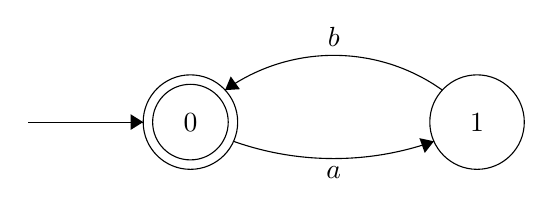
\begin{tikzpicture}[scale=0.2]
				\tikzstyle{every node}+=[inner sep=0pt]
				\draw [black] (30.5,-26.5) circle (3);
				\draw (30.5,-26.5) node {$0$};
				\draw [black] (30.5,-26.5) circle (2.4);
				\draw [black] (48.7,-26.5) circle (3);
				\draw (48.7,-26.5) node {$1$};
				\draw [black] (45.963,-27.721) arc (-70.47013:-109.52987:19.034);
				\fill [black] (45.96,-27.72) -- (45.04,-27.52) -- (45.38,-28.46);
				\draw (39.6,-29.32) node [below] {$a$};
				\draw [black] (32.698,-24.47) arc (125.49294:54.50706:11.887);
				\fill [black] (32.7,-24.47) -- (33.64,-24.41) -- (33.06,-23.6);
				\draw (39.6,-21.76) node [above] {$b$};
				\draw [black] (20.2,-26.5) -- (27.5,-26.5);
				\fill [black] (27.5,-26.5) -- (26.7,-26) -- (26.7,-27);
				\end{tikzpicture}
			\end{center}
			
			
			However, $ perm(A)=\{x\in \{a,b\}^* \mid \#a(x)=\#b(x) \} $ is not regular as we showed in class.\\
			\end{proof}

			\begin{claim}
				Regular languages are closed under cyclic permutations.
			\end{claim}
			Given a regular language $ B $, there exists a DFA $ M=\{Q,\Sigma,\delta, s,F\} $ such that $ L(M)=B $. We want to build an NFA that accepts the language of $ cyc(B) $.\\
			
			Intuitively, every string that is accepted by the DFA has a path on the automaton that starts from the start state and ends in some final state. Suppose this string is $ xy $, where $ x,y\in \Sigma^* $. Then we want to create an automaton that accepts the string $ yx $. To do this, the automata would need to accept the string starting from $ y $ and then `continue' to accept the rest of the string $ x $. Therefore we need the automata to be able to start at any state $ q $ in any path, inherit the paths the original final states and then `pick off' from the start state until it reaches $ q $.\\
			
			\newpage
			\noindent Formally, fix a state $ q\in Q $ and consider the automaton $ M_q $ comprised of two copies of $ M $, where 
			\begin{itemize}
				\item $ M_q:=\{Q_q, \Sigma, \Delta_q, S_q, F_q\} $
				\item $ Q_q:=\{p_q, p_q'\mid p\in Q\}$
				\item If $ \alpha\in Q, c\in \Sigma $ then $ \Delta_q(\alpha_q,c) :=\delta(\alpha,c)_q$ and $ \Delta_q(\alpha_q',c) :=\delta(\alpha,c)_q'$
				\item $ \Delta_q(f_q,\epsilon):=\{s_q'\} $ ($ \varepsilon $ transitions the final state of the first copy to the start state of the second)
				\item $ S_q:=\{q_q\}, F_q:= \{q_q'\}$\\
			\end{itemize}
			
			\noindent Now, we want an NFA that has the combined properties of all the automata $ M_q $ for all $ q\in Q $. Therefore, let $ M_N:=\{Q_N,\Sigma,\Delta, S_N,F_N\} $ and
			\begin{itemize}
				\item $ Q_N:=\bigcup_{q\in Q} Q_q $, $ S_N:=\bigcup_{q\in Q} S_q $, $ F_N:= \bigcup_{q\in Q} S_q $
%				\item $ \Delta(f_q,\epsilon):=\{s_q'\}$
				\item  For all $ q\in Q, \beta\in Q_N, c\in \Sigma\cup\{\varepsilon\}, $ $ \Delta(\beta_q,c) :=\Delta_q(\beta_q,c)$\\
			\end{itemize}
		
		\begin{theorem}
			$ L(M_N)=cyc(B) $
		\end{theorem}
		\begin{proof}
			Let $ xy\in B $. Then $ \hat{\delta}(s,xy)\in F$. Let $ \hat{\delta}(s,xy)= \hat{\delta}(\hat{\delta}(s,x),y):=f $ and $ \hat{\delta}(s,x):=\alpha $. Then 
			
			\begin{align*}
				\alpha_\alpha \in S_N &\implies \hat{\Delta}(S_N,y)\ni \hat{\delta}(\alpha_\alpha, y)
				\ni f_\alpha\\
				\hat{\Delta}(f_\alpha,x)&=\hat{\Delta}(\hat{\Delta}(f_\alpha,\varepsilon),x)\\
				&\supseteq \hat{\Delta}(s_\alpha',x)\\
				&= \hat{\Delta}_\alpha(s_\alpha',x)\\
				&\ni \hat{\delta}(s,x)_\alpha'\\
				&=\alpha_\alpha'\in F_N\\
			\end{align*}
			\begin{align*}
				&\implies \hat{\Delta}(S_N,yx)=\hat{\Delta}(\hat{\Delta}(S_N,y),x)\supseteq \hat{\Delta}(f_\alpha,x) \ni \alpha_\alpha'\in F_N\\
				 &\implies \hat{\Delta}(S_N,yx)\cap F_N \neq \varnothing \implies yx\in L(M_N)\\
				 &\implies L(M_N)=cyc(B)
			\end{align*}
		\end{proof}
\end{document}